% !TEX encoding = UTF-8 Unicode
%!TEX root = thesis.tex
% !TEX spellcheck = en-US
%%=========================================
\section{Experiment 1}
In this experiment, the aim is to find good values for crossover rate and mutation rate.

\subsection{Configuration}

\begin{center}
\begin{longtable}{p{5cm} p{7cm}}
\caption[Experiment configuration]{Experiment configuration} \label{tab:exp1_configuration} \\

\hline \multicolumn{1}{l}{\textbf{Parameter}} & \multicolumn{1}{l}{\textbf{Value}} \\ \hline 
\endfirsthead

\multicolumn{2}{c}%
{{\bfseries \tablename\ \thetable{} -- continued from previous page}} \\
\hline \multicolumn{1}{l}{\textbf{Parameter}} & \multicolumn{1}{l}{\textbf{Value}} \\ \hline 
\endhead

\hline \multicolumn{2}{r}{{Continued on next page}} \\ \hline
\endfoot

\hline \hline
\endlastfoot

Number of generations & 20 \\
\midrule
Fitness function & Local similarity \\
\midrule
Target sound & Drum loop \\
\midrule
Input sound & White noise \\
\midrule
Effect & Distortion and resonant low-pass filter \\
\midrule
Audio features & mfcc\_0, mfcc\_0\_\_derivative, mfcc\_1 \\
\midrule
Number of runs & 150 per configuration \\
\end{longtable}
\end{center}

\subsection{Fitness function}
The local similarity fitness function is based on the average euclidean distance between the feature vector of the target sound and the output sound in the k frames of the two sounds.

\begin{verbatim}
Function LOCAL_SIMILARITY(target, individual):
    total_euclidean_distance = 0
    for each k in range(num_frames):
        A = target.get_feature_vector(k)
        C = individual.get_feature_vector(k)
        total_euclidean_distance += EUCLIDEAN_DISTANCE(A, C)
    avg_euclidean_distance = total_euclidean_distance / num_frames
    return 1 / (1 + avg_euclidean distance)
\end{verbatim}

where \texttt{EUCLIDEAN\_DISTANCE} is $d(p,q)=\sqrt{(q_1-p_1)^2+(q_2-p_2)+...+(q_n-p_n)^2}$

\subsection{Results and evaluation}
Figure \ref{fig:exp1_heatmap} shows that one should avoid using a high mutation rate and a low crossover rate. Instead, one of the combinations inside the red region should do well. Bear in mind that the differences between pure yellow and lime green are small in this region, and that these small differences are not statistically significant. The variance could be reduced with more runs, but due to computational time, the number of runs per configuration was limited to 150. The yellow spot is probably a good configuration, albeit not necessarily the best. Muration rate = 0.6 and crossover rate = 0.7 are used in the following experiments.

\begin{figure}[h]
    \centering
    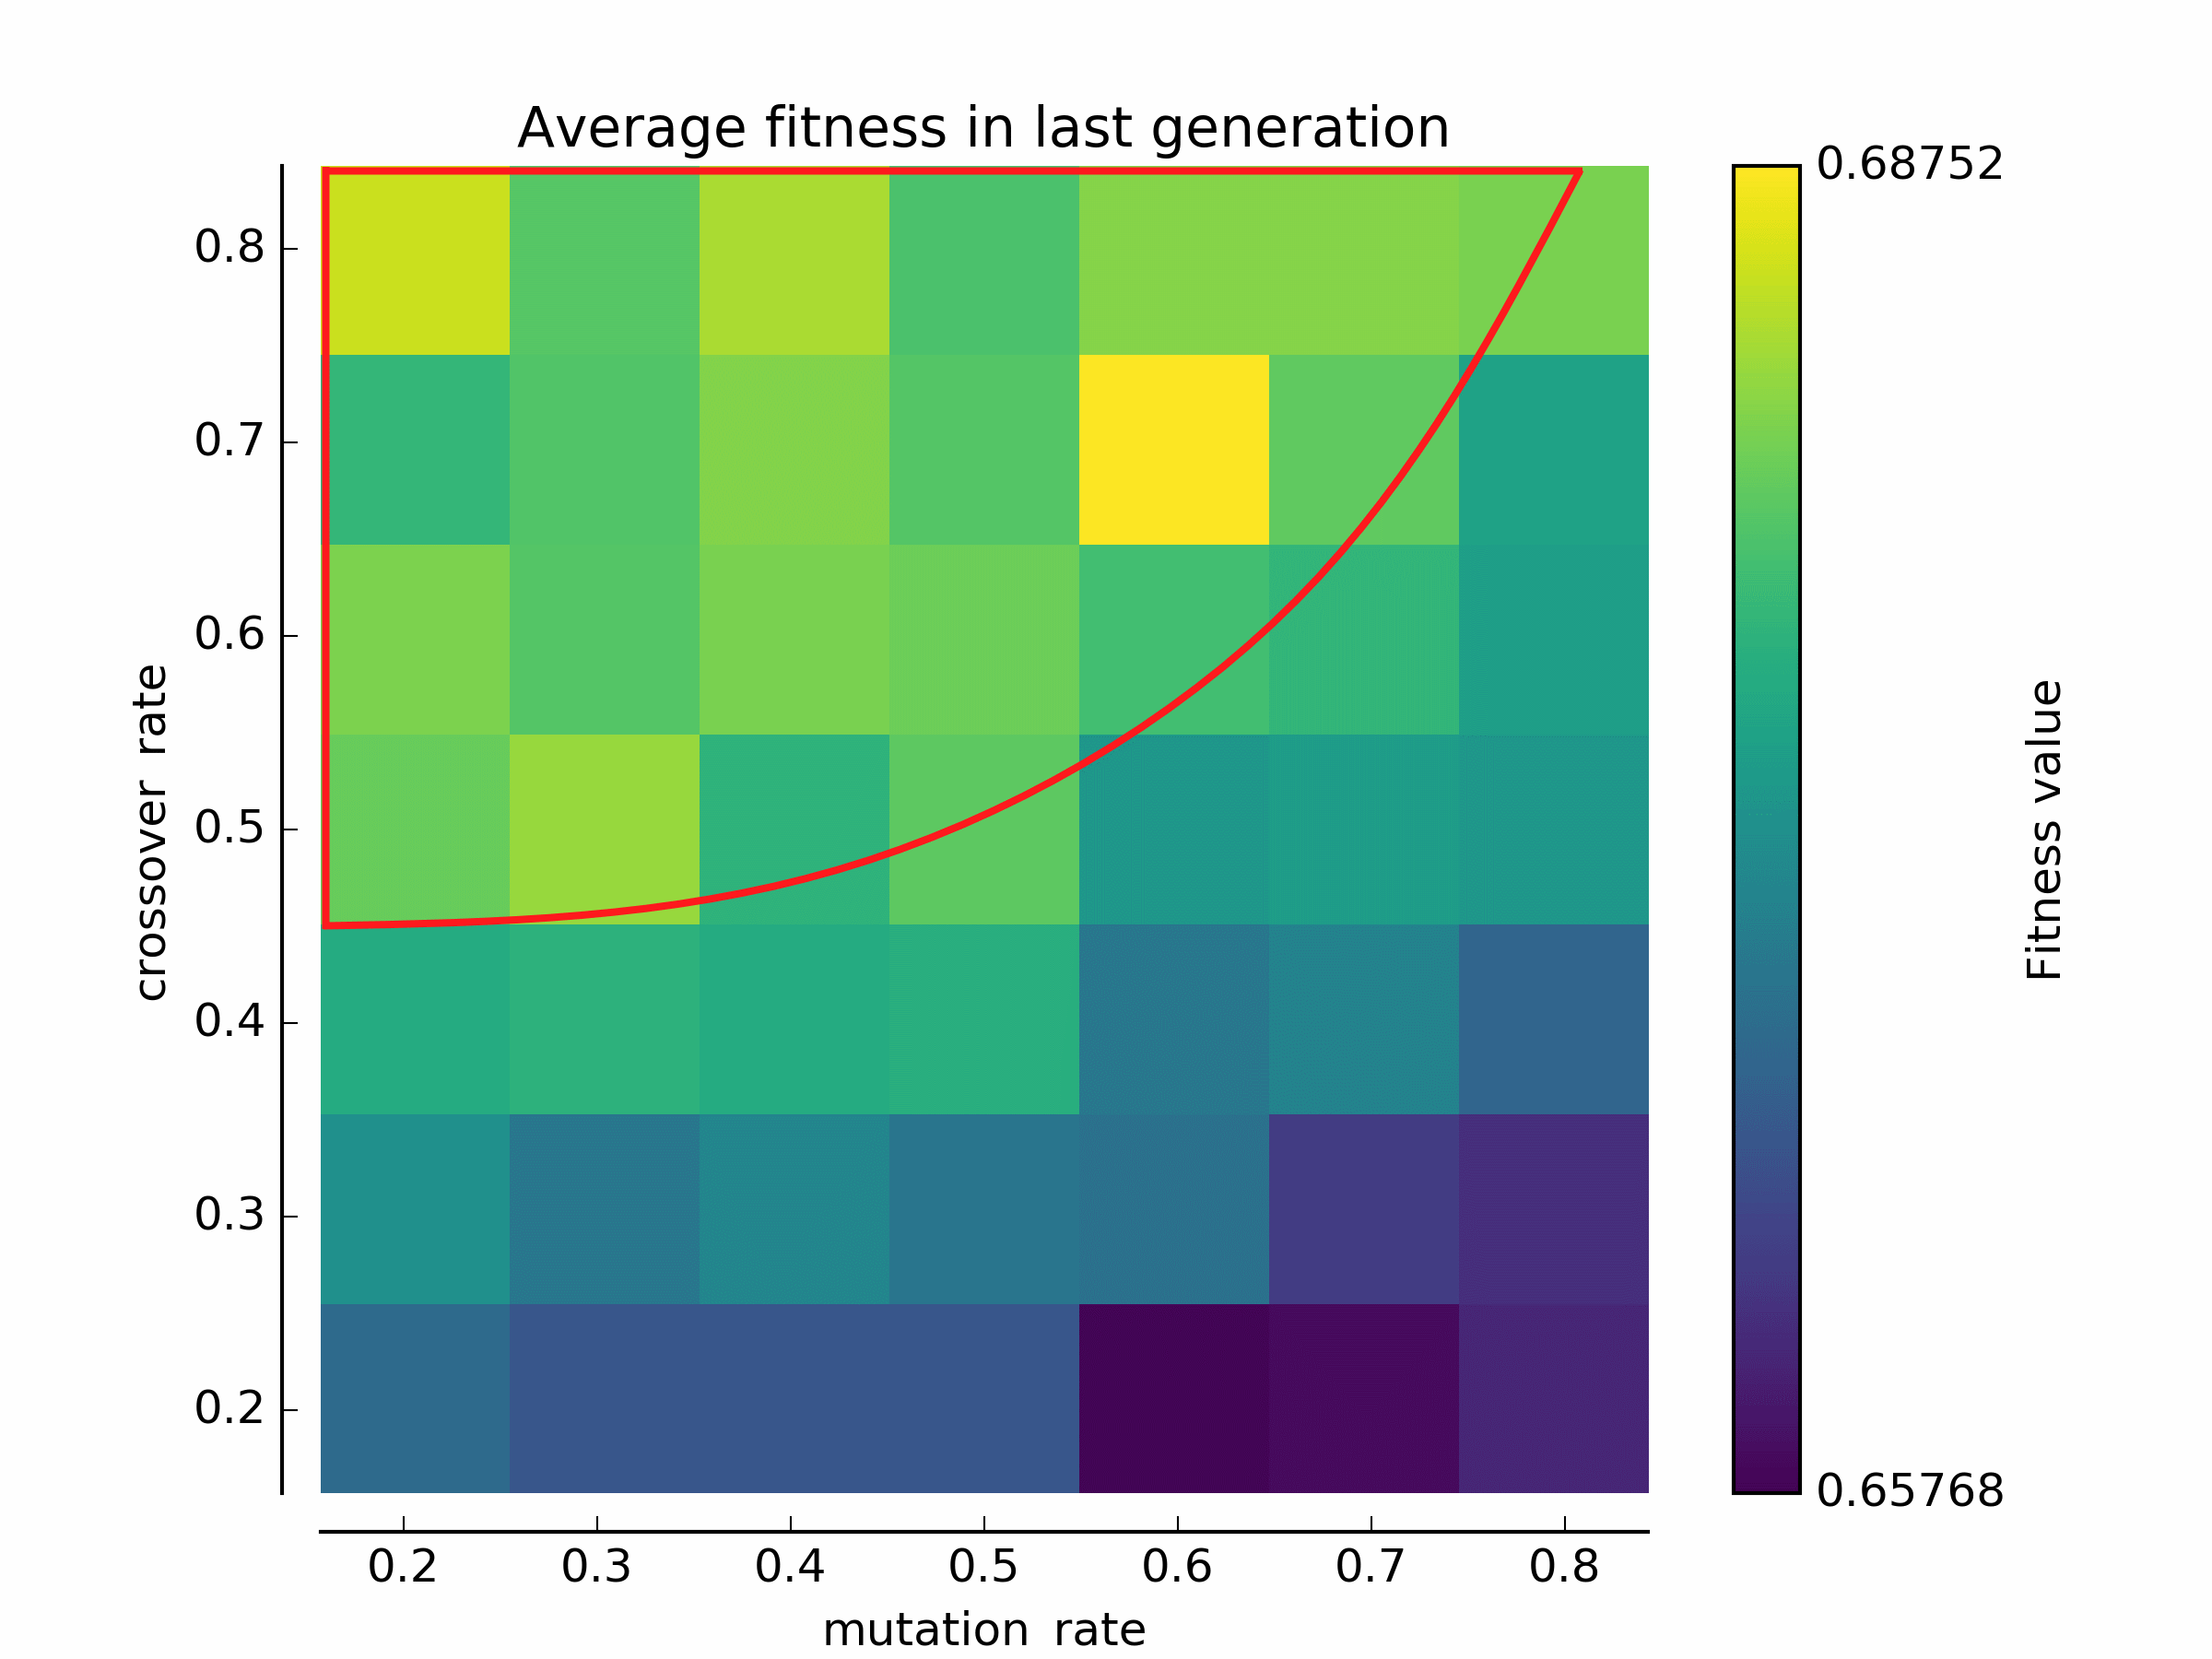
\includegraphics[width=0.99\textwidth]{grid_search_crossover_mutation_avg}
    \caption{Heat map with a red region, indicating the best configurations}
    \label{fig:exp1_heatmap}
\end{figure}